\RequirePackage{snapshot}
\documentclass{dsj}
\usepackage{amsmath}%,amsthm}
\usepackage[utf8]{inputenc}
\usepackage[main=english,spanish]{babel}
\usepackage{times}

\usepackage[style=science,article-title=true,doi=false,isbn=false,url=false,backend=biber, maxnames=50]{biblatex}
\addbibresource{bibliography.bib}

\usepackage{graphicx}

\usepackage{hyphenat}

\usepackage{nameref}
\newcommand{\beginsupplement}{%
\setcounter{table}{0}    \renewcommand{\thetable}{A\arabic{table}}     \setcounter{figure}{0} \renewcommand{\thefigure}{A\arabic{figure}}
}


\begin{document}

\footer{Footer Text}
\submitted{ - }

\title{Inventors' Explorations Across Technology Domains}

\author[*,1,2]{Jeff Alstott\email{alstott@mit.edu}}
\author[*,1,3,4]{Giorgio Triulzi\email{gtriulzi@mit.edu}}
\author[1]{Bowen Yan}
\author[1]{Jianxi Luo}

\address[1]{Singapore University of Technology and Design}
\address[2]{Massachusetts Institute of Technology, Media Lab}
\address[3]{Massachusetts Institute of Technology, Institute for Data, Systems, and Society}
\address[4]{United Nations University - MERIT}
\address[*]{These authors contributed equally to this work.}


\maketitle

\begin{abstract}
Technologies are created through the collective efforts of individual inventors. Understanding inventors' behaviors may thus enable predicting invention, guiding design efforts or improving technology policy. We examined data from 2.8 million inventors' 3.9 million patents and found most patents are created by ``explorers'': inventors who move between different technology domains during their careers. We mapped the space of latent relatedness between technology domains and found explorers were 250 times more likely to enter technology domains that were highly related to the domains of their previous patents, compared to an unrelated domain. The great regularity of inventors' behavior enabled accurate prediction of individual inventors' future movements: a model trained on just 5 years of data predicted inventors' explorations 30 years later with a log-loss below 0.01. Inventors entering their most related domains was associated with patenting up to 40\% more in the new domain, but with reduced citations per patent. These findings may be instructive for inventors exploring design directions, and useful for organizations or governments in forecasting or directing technological change.
\end{abstract}

\section*{Introduction}

Technology development and engineering design have been characterized as processes of creative transformation, recombination or synthesis of prior technologies and related knowledge into new creations \cite{Fu2013, Weisberg2006, Arthur2009, Hatchuel2009, Tang2013}. Highly-novel designs as well as knowledge production have been shown to arise from creative interdisciplinary combinations \cite{Reich2012, Fleming2001, Nooteboom2007, Arthur2009, Uzzi2013, Kim2016}. These empirical evidences have influenced innovation policies, which are increasingly encouraging inventors to develop a broad knowledge base and to span across technology domains \cite{Clough2004, Olson2013,EURAB2004}. However, little is known about how inventors explore across technology domains during their design efforts, such as whether there are typical patterns of exploration or patterns associated with higher outcomes. Understanding the general trends of inventors' movements and performance across domains may allow for better prediction of future invention, facilitate design-by-analogy inventive efforts \cite{Linsey2007, Linsey2012, McAdams2002} and enable more fine-grained innovation polices.


Do inventors preferentially explore domains of technology closely related to what they already know? What are the performance implications of movements into related versus unrelated domains? We can now address these questions thanks to accurate tracking of inventions' inventors \cite{Li2014} and quantitative measures of the relatedness between technology domains \cite{Alstott2017, Kay2014, Leydesdorff2014, Verspagen1997}. The relatedness of technologies and products is important for the outputs of firms \cite{Neffke2013, Bottazzi2010, Leten2007, Breschi2003}, cities \cite{Rigby2013}, regions \cite{Castaldi2015, Neffke2011, Frenken2007} and countries \cite{Hidalgo2007}: they are more likely to successfully generate an output in a new domain if it is highly related to their previous domains.
All of these entities, however, are composed of individual inventors, which have greater cognitive constraints than the organizations they make up. Here we study at scale how individuals' inventive behaviors are shaped by the relatedness of technology domains. 


We used data from 3,910,549 patents awarded by the United States Patent and Trademark Office between 1976 and 2010 to track 2,756,382 inventors as they patented their inventions. We found that inventors were far more likely to enter domains related to their previous work, and when they did so they patented more in the new domain. The great regularity of inventors' explorations across domains made their movements predictable, which enabled us to further create an accurate predictive model of inventors' future exploration, and allows for more informed interdisciplinary design efforts.



\section*{Aims}
Here we aim to measure, at scale, inventors' behavior as they explore different technology domains. We seek to find a quantification of how much technology domains relate to each other, and then use that information to build a predictive model of inventors' movements across domains. We will also evaluate if different types of movements are associated with different performance outcomes, using several dimensions of performance.


\section*{Literature Review}
Technological innovation is the process of producing effective solutions to engineering design problems. This process' characteristics have been studied by scholars of design science, creativity and innovation. These different branches of study have repeatedly concluded that high-impact inventions are generated from the creative combination of existing solutions 
\cite{Weisberg2006, Arthur2009, Hatchuel2009, Tang2013, Uzzi2013, Fleming2001, Hatchuel2003, Hatchuel2004}. The broad agreement on this view of the engineering design and innovation process has lead to the formulation of national and supranational science and technology policies that stimulate inventors to source knowledge from different technology and scientific domains \cite{Clough2004, Olson2013,EURAB2004}.

Combining prior knowledge from existing engineering solutions may not be easy, and the difficulty depends on the strength of the relatedness between different pieces of knowledge. We can characterize different technologies to be more or less similar in terms of how much their inventive process shares similar knowledge inputs and capabilities \cite{Alstott2017}. Inventors can leverage existing knowledge and existing design solutions from close and distant technology domains. Large-scale studies using data from patents and publications have shown that high-impact ideas usually come from domain-spanning work, often with the help of teamwork by groups of inventors \cite{Uzzi2013, Wuchty2007}. Uzzi et al. \cite{Uzzi2013} showed how atypical combinations of a few rarely co-cited scientific publications (often from different fields) and often co-cited papers (typically from the same field), increases the probability that the focal publication will be in the top $1\%$ of most cited publications. Other studies analyzing patent data broadly confirmed these findings \cite{Kim2016, Malva2014, Phene2006}. This suggests that high-impact ideas are unusual in that they combine popular conventional knowledge with pieces of knowledge that are usually consider to be cognitively unrelated. However, it is important to distinguish between the potential value of combining different knowledge and its actual realization. Using patent data, Fleming \cite{Fleming2001} showed how experimentation with new components of technical knowledge or new combinations of different pieces of knowledge leads to less useful inventions on average, but it also implies an increase in the variability that can result in both failure and breakthrough. 

Studies of engineering design provide more specific insights on how designers source knowledge to create novel artifacts.
Designers' work is strongly guided by their prior knowledge and experience \cite{Hatchuel2009, Hatchuel2003, Hatchuel2004}. On the other hand, designers also take inspiration from existing analogous solutions \cite{Chan2015, Reich2012, Shai2004}. However, designers' ability to mix very different strands of knowledge is constrained by their experience and their understanding of a set of scientific principles specific to their own field of work. Therefore, inventors are usually better equipped to incorporate existing knowledge from relatively similar analogous solutions in their creative process \cite{Linsey2007, Linsey2012}. In a recent text analysis of design concepts from a Web-based innovation platform, Chan et al. \cite{Chan2015} found that conceptually closer, rather than farther, sources of inspiration lead to more useful and appropriate ideas. However, several other case studies of specific design processes have shown how moderate \cite{Fu2013} or even distant knowledge inputs \cite{Tseng2008, Gentner1997, Wilson2010} can result in particularly novel ideas. For instance, Fu et al. \cite{Fu2013} performed an experiment in which patents that they classified as near or far analogous solutions to a given design problem were provided to designers as creative stimuli. They found that designers who were exposed to existing solutions from ``far" fields performed poorly, being unable to effectively integrate them into the design process. Similarly, designers who were only given ``near" patents produced design solutions with limited novelty, albeit with higher quality than the former. This shows how near fields are perceived to be more relevant sources of knowledge for the design process. However, the authors also discussed how stimuli of a moderate distance may be most conducive to the successful generation of highly novel solutions. Following this idea, Fu et al. \cite{Fu2013a, Fu2015} developed a method to measure how analogous two patented design solutions are to each other to help designers identifying the most useful stimuli for their creative process. The effect on design output of distance of external stimuli to the design problem were also studied by Chan et al. \cite{Chan2011} through a designed experiment similar to \cite{Fu2013}. They found a positive effect of far and less-common stimuli on novelty but also on the variability of a solution quality.

Taken collectively, these studies of engineering design suggest that, despite inventors' natural cognitive tendency to build on their prior experience and knowledge, designers may actually benefit from seemingly unrelated solutions. Mixing this new knowledge with what they have learned in the past in their own inventive history can lead to higher-novelty creations. This is likely to lead to failure in many instances, but a few solutions may prove to be breakthroughs \cite{Fleming2007a}. Designers can therefore benefit from tools that suggest to them where these potentially useful analogous existing solutions can be searched. One such tool could be a large-scale map of the space of technology domains and how closely they relate to each other. Such a map would help designers better understand how different knowledge can be mixed, foster diversification of inventive output and facilitate design-by-analogy.

The importance of mapping the technology space has lead to multiple attempts to use patent data to describe the space. Multiple measures have been developed to quantify how technology domains relate to each other. However, different measures produced different maps \cite{Kay2014, Leydesdorff2014, Schoen2012}. We have recently shown that all the most popular measures of relatedness are affected by several confounding factors (such as different domains having different ages or very different numbers of patents). When these factors are controlled for the different maps all collapse into much closer agreement, and these maps are on the whole very stable. \cite{Alstott2017}. Here we will use these methods to quantify how hundreds of domains relate to each other, and use that information to predict inventors' explorations across the space of technology domains.

A similar question has been addressed in the context of firms’ exploration and diversification into new product areas. Several studies showed that firms tend to preferentially diversify into related domains, though they can enter less related domains as well (see, for instance, \cite{Neffke2013, Leten2007, Nooteboom2007, Bottazzi2010, Breschi2003}). This is likely because firms’ explorations are much less constrained than individuals, most obviously through greater financial resources. However, firms can also have greater cognitive capacity, firstly by having multiple minds in the form of different employees, but also by the ability to simply acquire existing firms in operating in different domains. On a methodological point, previous studies on firm behavior have also used imperfect metrics of relatedness that may affect the correct inference of exploration behaviors, as shown by \cite{Bottazzi2010}. Hence, the present work addresses an important methodological and research gap on inventor’s search strategies and contributes to the design science community by examining the behavior of individual inventors, instead of management and organizations.


\section*{Methods}
\subsection*{Data}
Data on all patents granted between 1976 and 2010 by the United States Patent and Trademark Office (USPTO) were acquired from the USPTO's public data sets hosted by Google at https://www.google.com/googlebooks/uspto.html. 
Each patent contained three pieces of metadata used in the present analysis:
\begin{enumerate}
    \item The domain of the invention (its classification in the International Patent Classification system, at the 4-digit level, which has 629 classes.)
    \item Citations to other patents (if any)
    \item Who invented the invention (the name(s) of the patent's author(s), disambiguated with data from \cite{Li2014})
\end{enumerate}

More information about and interpretations of these metadata are included in \textit{Appendix}.

\subsection*{Measuring Technology Relatedness by Comparison to Random Expectation}\label{expectation_calculation}

We sought to predict what domain an inventor would explore next by quantifying how related other domains were to the domains of the inventor's previous patents. We called two domains ``related'' if they had an unusual amount of interactions in the patent record. Domains' patents can interact in many ways, such as by citing each other; such citations are a signal of technical proximity or knowledge coupling between domains \cite{Jaffe2002,Jaffe2016, Verspagen1997}. Thus we intend to measure the relatedness between two domains by how much patents from the two domains interacted with each other, such as by citing each other. However, citations (and many other ways that patents or domains can interact) are affected by more than just the relatedness between domains. As a simple example, if the domains both had many patents we would expect a large number of citations simply by chance. As a more complicated example, the age distributions of patents in each domain also affects citation rates between them, due to the peculiar shape of the age distribution of citations and the increasing average number of citations made by a newly granted patent, as shown in \cite{Alstott2017, Valverde2007, Jaffe2002, Hall2001}. These are examples of what we have called ``impinging factors'', which affect the measured interactions between technology domains but are not representative of the relatedness of technology domains.

We previously showed how to normalize several different measures of relatedness by controlling for many impinging factors at once \cite{Alstott2017}. This was done by comparing the empirical data of interactions ($I_{empirical}$) to what the data would be expected to look like by chance, holding several factors constant. To calculate how much two domains are expected to interact ($I_{expected}$), given observed properties such as their number of patents, we used link swapping to create 1,000 randomized versions of the historical record of the nearly 4 million patents. These randomized versions of history preserved the following features:

%(observed properties: $P$. $I_{expected} = f(P)$)
%(See \textit{Methods}), 

\begin{enumerate}
    \item the number of patents in each domain
    \item each patent's number of citations, both made and received
    \item each patent's portion of citations to patents in other domains (``cross-domain'' citations), both made and received
    \item each patent's exact citation age structure (e.g. a citation to a patent of granted in year 1980, and a citation received from a patent granted in 2002) 
    \item the age structure of each patent's cross-domain citations (e.g. the citation to a patent in 1980 was cross-domain, and the citation received from a patent granted in 2002 was same-domain)
\end{enumerate}

For each of these 1,000 versions of history we calculated the number of citations patents in each domain make to patents in each other domain. We could then measure if two domains interact more than the expectation: $I_{empirical}>I_{expected}$. Patents have numerous kinds of interactions to measure, but their deviations from expectation correlate: different measures give similar stories of how much two domains are related \cite{Alstott2017}. Here we measured interactions ($I_{empirical}$  and $I_{expected}$) simply by how much two domains' patents cite each other, using data from 35,129,936 citations (results using other measures of interaction are qualitatively similar and are shown in \textit{Appendix}).

If domains cite each other more or less than expected, this could be due to noise: the expectation $I_{expected}$ has variance, as could the influence of latent relatedness. We increased our confidence that two domains were related through repeated samples: using patents awarded each year from 1976 to 2010 we counted how many years $I_{empirical}$ was greater than $I_{expected}$. We expressed this count as a percentage, $R$, which was our measure of relatedness (Fig. \ref{R_definition}). Pairs of domains with high $R$ persistently interacted more than expectation, and were interpreted as more likely to be related. The majority (64\%) of domain pairs always had fewer citations than expectation ($R=0$)
, such as ``semiconductors'' to ``hydraulics'' (Fig. \ref{R_definition}, red line). Just $0.02\%$ of domain pairs always had more citations than expectation, such as ``semiconductors'' to ``static info storage'' (Fig. \ref{R_definition}, blue line). 

\begin{figure*}
\includegraphics[width=1.3\textwidth]{figs/R_definition.pdf} 
\caption{\textbf{Three examples of how relatedness, $R$, was calculated.} Each year citations to patents in the Semiconductors domain from patents in other domains were counted and compared to the quantity expected by random chance, given all domains' number of citations and other factors. $R$ was the portion of years that the number of citations was above expectation. 
}\label{R_definition}
\end{figure*}

\subsection*{Measuring the Relatedness of an Inventor’s Previous Domains to Unentered Domains}

With a measure of the relatedness between domains in hand, we then quantified how much an inventor’s existing knowledge was related to any specific domain. This was done through simply identifying every domain in which the inventor had previously patented, and then taking the mean R between those domains and the specific domain in question (Fig. \ref{Inventor_R_Diagram}). This quantity was calculated for every domain the inventor had not patented in. This quantity was calculated initially only accounting for the inventor’s first domain, and then recalculated every time the inventor patented in a new domain. This mean R was the measure used for models predicting inventors’ movements and performance (see below). Note that for these models the R used was the R as measured in the year immediately before the inventor filed their patent in a new domain, and so it did not include information about the inventor’s new patent, or indeed any future patents.

\begin{figure*}
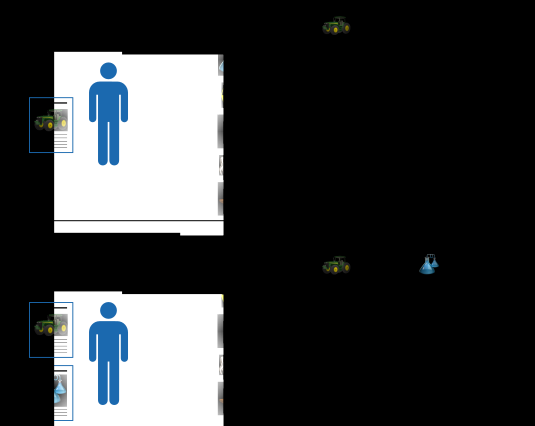
\includegraphics[]{figs/Inventor_R_Diagram.png} 
\caption{\textbf{An inventor's $R$ to an unentered domain was the average of the $R$ to the domain from each of the domains in which they had previously patented.}
Top) A diagram of an inventor before their first move. Since the inventor had patented in only one domain, the inventor's $R$ to each unentered domain was the same as the $R$ from that one domain. 
Bottom) A diagram of the same inventor before their second move. At this point the inventor had patented in two domains, so the inventor's $R$ to each unentered domain was the mean of the $R$s from the two domains.
Actual technology domains were very fine-grained (examples shown in Fig. \ref{movement_case}).
}\label{Inventor_R_Diagram}
\end{figure*}

\subsection*{Predictive Model}
Each time an inventor patented in a new domain we sought to predict what the domain would be. 
We created a predictive model that relied on the following data:
\begin{itemize}
    \item the mean R of the entered domain to the inventor’s previous domains
    \item the popularity of the entered domain (the number of patents granted in the domain in the year before the inventor patented in it)
    \item whether the inventor’s previous patents had cited patents in the entered domain
    \item whether the inventor’s previous co-authors had patented in the entered domain
\end{itemize}

Aside from R, the other factors are clearly potentially relevant to an inventor’s behavior. The popularity of the entered domain is meant to control for both the probability that an inventor’s patent is classified (or misclassified) into a large technology class just by random chance, as well as account for the possibility that inventors chase hot topics, regardless of its relatedness to their previous work. Information on the inventor’s co-authorship network is included to account for the possibility that the inventor had prior personal connection with authors in a newly entered domain, which may facilitate exploration. Empirical evidence that research is increasingly done in teams \cite{Wuchty2007}, has led to speculations of a growing need to rely on inter-domains knowledge across team members to achieve high impact (see for instance \cite{Borner2010} and \cite{Fiore2008}). This may motivate inventors to enter domains in which they know previous co-authors. The inventor’s previous citation(s) to a domain seeks to measure the existence of a personal knowledge bridge between the inventor’s prior work and a domain, which could influence the inventor’s exploration decisions more than the overall relatedness between domains. Such a personal bridge may exist due to several unobserved factors, such as the inventor’s educational background or personal connections with colleagues that have not co-authored the inventor’s previous work, as suggested by \cite{White2004}

The predictive model was created by identifying all the domains the inventor had not yet entered, then calculating $p(\text{entry})$ for each domain using a naive classifier:
\begin{align}
p(\text{entry}) \quad \sim & \quad  p(\text{entry}|R) * p(\text{entry}|\text{popularity})  \nonumber\\
&\quad * p(\text{entry}|\text{co-authors}) * p(\text{entry}|\text{citations})
\end{align}


$p(\text{entry})$ for each domain was thus a function of its mean $R$ to each of the inventor's previous domains, the popularity of the domain, whether the inventors had co-authors previously active in the domain, and whether the inventor's previous patents had citations to patents in the domain. For each of these variables $x$ we estimated $p(\text{entry}|x)$ by simply creating a histogram from historical data (this created a discrete naive classifier, discussed further in \textit{Appendix}). For co-authors and citations this histogram had only two bins: ($p(\text{entry}|\text{had co-authors active in domain})$ vs. $p(\text{entry}|\text{no co-authors active in domain})$) and ($p(\text{entry}|\text{had citations to patents in domain})$ vs. $p(\text{entry}|\text{no citations to patents in domain})$). For popularity, we created a histogram with $500$ bins (from popularity percentile rank $0$ to rank $100$, in intervals of $0.2\%$). Similarly, for $R$ we created a histogram of with $26$ bins ($R=0$, plus $25$ bins evenly spaced up to $R=1$). $p(\text{entry}|x)$ was then taken to be the $p(\text{entry})$ for the bin that $x$ was in. We calculated $p(\text{entry}|x)$ for each year individually, using data from 1976 up through that year. Each inventor exploration was predicted using data only up through the year before the year the inventor applied for a patent in a new domain.

\subsection*{Performance Models}
Given that the next domain to enter could be predicted, one would be further interested in predicting the inventor's performance in the new domain. We modeled inventors' performance as patent and future citation counts when they patented in a new domain as a function of the properties of the domain and each individual inventor's history. These properties included:
\begin{itemize}
    \item the mean $R$ of the entered domain to the inventor's previous domains
    \item the popularity of the entered domain (the number of patents granted in the domain in the year before the inventor patented in it)
    \item the number of times the inventor's previous patents had cited patents in the entered domain (if any)
    \item the number of times the inventor's previous co-authors had patented in the entered domain (if any)
    \item the inventor's previous rate of producing patents (which has been shown to correlate with inventor's future patenting rates \cite{Conti2013})
\end{itemize}

These properties were combined into a vector, $\vec{x}$, and the outcomes were modeled as a function of this vector, $f(\vec{x})$.

Patent and citation counts were modeled as generated from a negative binomial distribution, a classic count model with a variance that can be much larger than the mean. The negative binomial had the form:

\begin{equation}
    p(\text{count}|\mu, \phi) = {\text{count} + \phi -1 \choose \text{count}} \left(\frac{\mu}{\mu+\phi}\right)^{\text{count}} \left(\frac{\phi}{\mu+\phi}\right)^{\phi}
\end{equation}

where $\mu$ is the mean and $\phi$ is the overdispersion parameter (which determines the variance). We set $\mu$ as a function of $\vec{x}$ and a baseline outcome: the average number of patents or citations received by all explorers who entered the same domain in the same year. This function had the form $\mu = e^{\beta \vec{x}}*\text{baseline}$. Thus, for each property $x_i$ in $\vec{x}$, $\beta_i$ reflected how much $x_i$ was associated with increasing or decreasing performance relative to the baseline of other explorers.

We used Bayesian inference to find the most credible values of the parameters $\beta$ and $\phi$, given the data and Gaussian priors for both ($\beta$ priors: normal distributions of mean 0 and standard deviation 2. $\phi$ prior: a gamma distribution with parameters $\mu_{\phi}^{2}/var_{\phi}$ and $\mu_{\phi}/var_{\phi}$, where $\mu_{\phi}$ and $var_{\phi}$ also had normal priors of mean 0 and standard deviation 2). Fig. \ref{count_model_parameters} shows the resulting posterior distributions for $\phi$ and for each $\beta_i$ for each property $x_i$. These posteriors were calculated using Hamiltonian Monte Carlo sampling, as implemented in the software package \textit{Stan} \cite{Carpenter2016}. We sampled the posteriors with 50 chains of 300 iterations of warm-up and 300 iterations of sampling, thinned down to 500 uncorrelated samples in the posterior. 

To assess if these count models were well-specified to the data, we used posterior prediction for each entry to calculate the models' 95\% credible interval for the explorer's number of future patents or citations in the domain. The observed patent and citation counts were within the models' 95\% credible interval approximately 95\% of the time (patents: 97.7\%, citations: 96.6\%).

When analyzing and modeling performance we only included the entries up to 2005 (as opposed to 2010), to ensure each entry had at least 5 more years to observe the inventor's subsequent performance.

\subsection*{Data Availability}
All data and code for analyses, including generating figures, is contained in the Supporting Information. All code is also hosted at \url{https://github.com/jeffalstott/inventorexploration}.

\section*{Results}

\begin{figure}
\begin{center}
\includegraphics[width=\textwidth]{figs/movement_frequency.pdf} 
\end{center}
\caption{\textbf{Inventors regularly explore across technology domains.} The probability that an inventor's next patent was in a previously unentered technology domain, given the number of patents the inventor already had (double logarithmic axes).
}
\label{movement_frequency}
\end{figure}

Most (60\%) inventors patented only once, but 84\% of patents were made by repeat inventors with more than one patent. Inventors' patents were classified into 629 domains of technology by domain-expert patent examiners (see \textit{Appendix}). We could thus track as repeat inventors patented in one technology domain, such as ``semiconductors'', and then later patented in another domain, such as ``photography.'' We call this ``exploring'' or ``entering'' a new domain and inventors who do this ``explorers.'' 71\% of repeat inventors were explorers, and they were granted 77\% of patents. Explorers made a total 1,763,920 entries, and 56\% of patents were granted to an explorer who had entered the patent's domain from elsewhere. An inventor's probability of exploration was related to how many prior patents the inventor already had, with a form well-described by a power law 
(Fig. \ref{movement_frequency}). Heavy-tailed drop-offs in humans' exploratory behavior occur in other domains \cite{Brockmann2006,Deville2016} and indicate that inventors' apparent exploratory movements are not just due to erratic classification of patents (discussed in \textit{Appendix}).


When an inventor entered a new domain, we measured the mean $R$ from the inventor's previous domains to each of the domains they had not yet entered (the values of $R$ were calculated using only data from patents awarded up to the year \textit{before} the inventor applied for the patent, and thus did not include data from the inventor’s new invention). We found that inventors were far more likely to enter domains with high $R$; the probability of entering a domain with $R=1$ was 250 times higher than entering a domain with $R=0$ (Fig. \ref{R_pdf}A). Accordingly, the bulk of inventors' moves (92\%) were between pairs of domains linked by $R>0$, even though just 36\% of pairs were so linked (Fig. \ref{R_frequencies_in_network_and_entries}; a portion of these linked pairs are visualized in Fig. \ref{movement_case}). 

The tendency to enter a domain with high R was not the only factor that predicted inventors’ movements. If a domain was particularly popular, inventors were more likely to enter into it (Fig. \ref{R_pdf}B). Additionally, inventors were more likely to enter a domain if they had a more personal connection to it, such as by having had co-authors with prior patents in the domain, having had patents that cited patents in the unentered domain, or particularly having had both (Fig \ref{R_pdf}C). However, while both popularity and personal connections increased the probability an inventor would enter a domain, a higher R raised that probability further (Fig. \ref{R_pdf}B-C). 

\begin{figure*}
\includegraphics[width=1.3\textwidth]{figs/R_pdf_horizontal.pdf}
\caption{\textbf{Inventors were far more likely to explore a domain if it was related to their previous work.}
A) The probability density function of how likely an inventor was to move to a domain, given its mean $R$ to the inventor's previous domains.
B) As A, conditional on the popularity of the domain (the number of patents in the domain in the previous year).
C) As A, conditional on whether the inventor had previous co-authors who had patented in the domain before working with the inventor, and whether any of the inventor's previous patents had citations to the domain.
}\label{R_pdf}
\end{figure*}


\begin{figure}[]
\begin{center}
\includegraphics[width=\columnwidth]{figs/prediction_ranks.pdf}
\end{center}
\caption{\textbf{Inventors' explorations were predictable.} When each inventor moved, a naive predictive model ranked the inventor's unentered domains in order of their probability to be entered. The model had been trained with patent data from 1976 up to 1980 (blue), 1990 (green), or 2000 (red). Regardless of the model used, the domain actually entered was typically high on the prediction list. Perfect prediction: $1.0$,  Random prediction: $0.5$. Other measures of predictive power: c-statistic $>0.9$, log-loss $<0.01$ (Fig. \ref{prediction_quality_other_measures})
}\label{prediction_ranks}
\end{figure}

The regularity of inventors' movements allowed for predicting individuals' future explorations across domains. We applied our predictive model (a discrete naive classifier), described above, to calculate the probability of an inventor entering a domain, as a function of $R$, popularity, co-authors and citations. Each time an inventor moved we created a list of their unentered domains, ranked from most probable to least probable to be entered. Perfect prediction would always put the domain actually entered at the top of the list, and random prediction would put it in the middle of the list on average. The predictive model consistently put the domain actually entered within the top 2\% of the list half the time, and within the top 7\% of the list on average (Fig. \ref{prediction_ranks}). Other measures of predictive power include a c-statistic over 0.9 and log-loss below 0.01 (Fig. \ref{prediction_quality_other_measures}). Even when the model was trained only using data up to 1980, it accurately predicted inventors' movements in 2010, 30 years into the future. The persistent prediction indicates that the relationships captured in this model were stable for over 30 years. Thus, the model will likely retain predictive power going forward.

Knowledge production is increasingly done by teams, and teamwork is important for combining knowledge from different fields \cite{Wuchty2007,Uzzi2013}. About half of explorers had a ``guide'': their first patent in the entered domain had a co-author that had patented in that domain before. Explorers were more likely to have a guide if they entered a domain with high $R$ rather than low $R$ (Fig. \ref{p(Guide)_by_R}; 70\% for $R=1$ vs. 47\% for $R=0$). Regardless of the explorer’s R to the domain entered, they were typically accompanied by 1 co-author who was also an explorer (Fig. \ref{N_co-authors_by_R}). For the many explorers without guides, if the explorer had a higher $R$ to the entered domain they were more likely to have a co-author that, while not a guide, also had a higher $R$ to the new domain (Figs. \ref{p(Co-Author_R_Greater_than_X)_by_R}, \ref{p(Co-Author_R_within_X)_by_R}). Thus, those explorers entering domains with higher $R$ were more likely to be part of teams with experience in or connection to the domain.

\begin{figure}%[p]
\includegraphics[width=\columnwidth]{figs/p(Guide)_by_R.pdf} 
\caption{\textbf{Explorers were more likely to have a guide if they entered a domain with high $R$ to their previous patents}. }\label{p(Guide)_by_R}
\end{figure}

\begin{figure}%[p]
\includegraphics[width=\columnwidth]{figs/N_co-authors_by_R.pdf} 
\caption{\textbf{The number of co-authors an explorer had on their first patent in a new domain increased with $R$, while the number of co-authors who were also explorers to the domain was largely unassociated with $R$}. }\label{N_co-authors_by_R}
\end{figure}



\begin{figure*}%[p]
\includegraphics[width=1.3\columnwidth]{figs/p(Co-Author_R_Greater_than_X)_by_R.pdf} 
\caption{\textbf{Explorers' first patent in an entered domain was more likely to have co-authors with higher $R$ to the domain if the explorer had a higher $R$ themself}. When an explorer entered a new domain, their first patent in the domain could have co-authors, and those co-authors could also be explorers to the domain. Of those fellow explorers, we can ask the probability that at least one of them will have a high $R$ to the entered domain, with varying thresholds for what is a ``high'' $R$ (different colored lines). The probability of having a high $R$ co-author was a function of the explorer's own $R$ (x-axis). Note that the plotted lines terminate once the explorer's own $R$ is above the threshold; thus, this is the probability of an explorer having a co-author with a higher $R$ than their own. The data presented is for the 45\% of explorers that did not have a guide on their entering patent (a co-author who had previously patented in the entered domain).}\label{p(Co-Author_R_Greater_than_X)_by_R}
\end{figure*}


\begin{figure}[]
\includegraphics[width=\columnwidth]{figs/patents_citations_and_citations_per_patent_with_models.pdf}
\caption{\textbf{Inventors had higher total performance when they entered domains more related to their previous work, but lower average citations.} 
Blue) An explorer's number of additional patents in the entered domain after the entering patent.
Green) The number of citations those patents received
Red) The average number of citations per patent. All values are expressed relative to entering a domain with $R=0$.
Dashed lines: empirical averages, binned by $R$ in 11 bins from 0 to 1.
Solid colors: association of $R$ with performance, as inferred from models that accounted for other factors (Line: median expectation of performance, assigning all empirical entries a given value of $R$ and holding all other parameters constant at their empirical values. Shading: 95\% credible interval). Parameter values for these models are shown in Fig. \ref{count_model_parameters}
}
\label{performance}
\end{figure}

Where an inventor explored had ramifications for their future performance.
Inventors who entered domains with high $R$ to their previous domains went on to have more patents in the new domain (Fig. \ref{performance}, blue). These patents had more total citations (Fig. \ref{performance}, green), but because the number of future citations grew with $R$ slower than the number of future patents, the average citations per patent was lower for explorers who entered a domain with higher $R$ (Fig. \ref{performance}, red). These results suggest that inventors face a performance trade-off. They are more likely to be highly productive when they explore a domain related to their prior knowledge. But the average quality of their inventions in a newly explored domain is likely to be higher if they domain is less related to their previous creations.


We tested if these relationships between $R$ and performance held while accounting for other factors by applying Bayesian inference to fit the model of explorers' future performance that we introduced in \textit{Methods}. In addition to $R$, this model included: the entered domain's popularity; personal connections like previous co-authors' patents in the domain and the explorer's previous citations to the domain; whether the entering patent had a guide; the entering patent's number of co-authors; the explorer's previous productivity (number of patents per year since their first patent). After accounting for these other factors, the relationships between $R$ and performance persisted (Fig. \ref{performance}, solid lines).




\section*{Discussion}

\begin{figure*}
\includegraphics[width=1.3\columnwidth]{figs/Case_Study_patents.png} 
\caption{\textbf{Three instances of inventors exploring a new technology domain}. Left) In 1996 three inventors, Wim B., Sandra S., and George S., all entered the domain of ``heterocyclic compounds'' (chemicals with a ring of carbon and non-carbon atoms). They had all patented in only one domain previously, had no co-authors who had previously patented in the new domain, and their patents had not cited the new domain. Their performance in the new domain was related to the $R$ of the new domain with their previous experience (table). Right) Maximum spanning tree of the full set of all 629 technology domains and their $R$ to each other. To aid visualization, a community structure is highlighted, and some of the larger domains are labeled.
Link width: $R$ between two domains.
The node sizes and link widths are visualized using all patent data from 1976 to 2010, but the rank order of both moved little during the years visualized.
}\label{movement_case}
\end{figure*}

We quantified the relatedness of technology domains and demonstrated its relevance to inventors' movements and performance, at scale. Using relatively simple models we were able to effectively predict inventors' explorations and describe their multi-dimensional performance outcomes. 
Inventors' movements across domains of technology are predictable because the moves are shaped by where the inventors have been before: domains that are related to an inventor's previous work are explored more frequently. These movements to highly related domains also yielded more patents (as was the case of inventor Wim B., Fig. \ref{movement_case}). The entering and repeated patenting in related domains may be because related domains are comparatively easy to enter. The ease of entry likely stems from the inventor possessing relevant knowledge and skills, but it may also be due to the inventor having access to physical equipment and other external resources that affords the exploration. 
Exploring a less related domain is likely harder, which is why fewer inventors successfully do so, and even those who do enter don't typically patent as much (as with Sandra S. and George S., Fig. \ref{movement_case}). 



Patent counts are one measure of performance, but not all patents are equal in value: patents' citations are an indicator of how valuable the patented technology was for the economy or society, and that value likely increases superlinearly with the number of citations a patent receives \cite{Trajtenberg1990,Albert1991,Harhoff1999,Hall2000,Gambardella2008}. Inventors who explored domains with high $R$ received more total citations, but the citations per patent were lower; depending on the exact value of citations per patent, it is thus possible that the rare inventors who successfully entered domains with lower $R$ created inventions with more value. Creating more value from spanning disparate domains has been suggested by prior studies \cite{Nooteboom2007,Nooteboom2000}, but the observed increase in citations per patent after moving to lower $R$ has a selection bias: those rare inventors who cross the chasm to unrelated domains are likely particularly talented or well-supported, and we do not observe the less-resourced inventors who tried to enter a less-related domain and failed to patent. Thus, the higher citation per patent after exploring a lower $R$ domain could be entirely artifactual. Future studies with different data will be necessary to address this selection bias and assess the expected value of attempting to enter a less related domain.

A patent’s broader impact could potentially be seen by more than just its citations received. In those rare cases where an inventor who has previously patented in a domain X creates an invention in a new domain Y that had low R with X, we hypothesize that it could create a lasting connection between those domains. This may happen when the invention created a new generic technique that reorganized the working system of an artifact, as suggested by a recent model by \cite{Masson2017}. A truly high-impact patent would then lead to the whole population of inventors seeing more connections between X and Y, and that this would lead to the R between the two domains to increase. Measuring such step-changes in R and their potential antecedents in individual patents is an opportunity for further research.

\subsection*{Predictive power's implications to practitioners and policymakers}
The predictive model of inventors' explorations was so accurate over several decades because inventors' movements are very regular. A large component of this regularity is the network of relatedness between technologies, a portion of which is mapped in Fig. \ref{movement_case} and the entirety of which is included in \textit{Supporting Information}. This network map and the prediction that it affords may be useful to inventors, company managers and policymakers.

The technology relatedness map and performance prediction models may aid engineering designers in their assessment of possible exploration opportunities. Designers can use the map to identify domains that they can most feasibly explore for new opportunities, given their own personal history of which domains they have prior experience in. The map can also be used to search for interesting domains that are far from a designer's previous  domains. In this case, the performance models can help guide the search by estimating performance implications and trade-offs associated with exploring distant domains. Taken together, the technology relatedness map and the prediction models form a useful tool that can guide designers in their search for inventing opportunities, by helping them make more informed decisions. 

Many inventors work for research labs or research divisions of companies, and in many instances an inventor's exploration of a new domain may be the result of a strategic managerial decision by the employer.
However, inventors cannot be readily repurposed to new research projects in any arbitrary domain. Instead, their knowledge and experience is most readily transferable to the few related domains that are related to their previous knowledge, and those domains can be identified with the technology relatedness network map. Related domains are where inventors are more likely to be able to invent and to invent successfully, at least as measured by higher average levels of patenting. How to best pursue outlier performance, such as radical innovation, may yet require other strategies \cite{Uzzi2013,Kim2016}. The relatedness network map can instead be used by companies, research laboratories and research intensive government agencies to identify their workforce's expertise and where that expertise may be most readily reallocated for new projects.

Likewise, the network map of technology relatedness may also be useful for policymakers trying to foster interdisciplinary collaboration, as it can tell them which domains are likely to work well together. This may help the practical implementation of policies advocating for interdisciplinary science and technology \cite{Clough2004, Olson2013, EURAB2004}. Information on which domains are related to which others may also be useful for policymakers trying to grow a target domain. The target domain could be a technology that a lagging country is trying to catch up to the level of another country; the target domain could also be a technology that is nascent around the world and the objective is to grow the domain for global benefit. In either case, it may be possible to deliberately coax inventors from related domains into the target domain to increase the manpower and invention in the technology. Whether inventors typically respond successfully to such coaxing by policymakers, or reallocation by company managers, is a question deserving further research.


The better understanding of individual inventors' behavior achieved here may also enable expanded research on principles of technology development. It would be possible to model inventor population dynamics within and across domains, or to measure how technological shocks propagate between related domains across the technology space. Understanding how individuals' choices lead to aggregate outcomes may thus be a basis for predicting broad technological change.


\section*{Acknowledgements}
JA, GT and JL designed the study. BY collected the data and visualized the networks. JA and GT developed and performed the analysis. JA, GT and JL wrote the paper. We thank César Hidalgo, François Lafond, Aditya Mathur, Chris L. Magee, James Savage, Kristin Wood and Hyejin Youn for helpful discussions.

\section*{Financial Support}
This work was supported by the SUTD-MIT International Design Centre (IDG31300112), the Singapore Ministry of Education Tier 2 Academic Research Grants (T2MOE1403) and the SUTD-MIT Postdoctoral Programme.

\printbibliography[]%heading=none]

% \clearpage
\newpage
\beginsupplement
\newrefsection

\title{Appendix}
\maketitle

\section{Data}

\subsubsection*{The domain of the invention (classification)}
For a patent to be granted, the invention described in the application must be considered sufficiently novel and non-obvious by a patent examiner who is an expert trained in the subject matter. To ensure that a patent is examined by an examiner who is actually an expert in the domain, it is necessary to match the patent with a domain, and then the patent can be assigned to the correct patent examiners. Similarly, in order to ensure that the patent describes an invention that is novel, the patent examiner should be able to access a set of patents within the domain of the patent, so as to compare them. For this purpose it is also useful to have each patent matched with a domain, for ease of finding past patents that are relevant and for being found as relevant in future examination of other patents. For these purposes, patent examiners classify patents into technology classifications systems. Individual patents' classifications can be and frequently are updated throughout the examination process, as the patent examiners have incentive to classify the patent as accurately as possible and to update the classification if it is inaccurate. Such classification updating can also occur once the patent is awarded: if a new domain of technology arises (e.g. 3D printing), a new technology class is eventually added to the classification system \cite{Lafond2017}. At this point, the USPTO goes back through all previously granted patents to re-classify those that belong to the newly-recognized technology domain. The reason for this re-classification is so that these older patents will still be found during future examinations of patents in the newly-recognized domains. Patent classification is thus a domain-expert-curated, repeatedly-updated assessment of what domains best describe millions of inventions. 

Patent offices around multiple technology classification systems. We used patent class data from the International Patent Classification system (IPC), curated by the World Intellectual Property Organization. Like most technology classification systems, the IPC is hierarchical: There are sections (e.g. `B: Performing Operations; Transporting') divided into classes (`B64: Aircraft; Aviation; Cosmonautics') divided into sub-classes (`B64C: Aeroplanes; Helicopters'). We used the sub-classes at the ``4-digit'' to represent the technology domains, of which there were 629. We took each patent's main classification at the 4-digit level to be the technology domain of that patent. 


The hierarchical classification system goes to further levels of detail, and it is conceivable to go deeper into the hierarchy to perform the present analysis with a higher-resolution description of technology domains. However, the predictive model of inventors' explorations involved retaining data not just on each domain that an inventor entered, but also all the domains that they did not enter. Keeping track of over 600 domains for each such move pushed the limits of computational tractability, and keeping track of thousands or tens of thousands of domains for each move would go beyond what is computationally feasible at present. 


\subsubsection*{Citations to other patents}
Patents typically contain citations to other patents, and the purpose of these citations to highlight the limits of what the patent can claim as novel intellectual property. For example, if a patent describes a telescoping fishing rod, it may cite a patent for a non-telescoping fishing rod and another patent using a telescoping mechanism in another context. This would make clear that the patent does not have claims to the ideas of fishing rods or telescoping mechanisms, but to specifically the telescoping fishing rod. Patent citations have been studied for decades as a signal how inventions build on other inventions \cite{Jaffe2016}. There remains questions of how much individual inventors are actually aware of these other inventions during their own invention process, as the most citations are not made by the inventors themselves, but by lawyers and patent examiners \cite{Alcacer2006, Criscuolo2008}. At the very least, it is clear a citation between two patents indicates that they describe inventions that are related in some way. We use citations as a signal of relatedness between technology domains, though that signal must be extracted from spurious factors  (described below).%(described in section \ref{expectation_calculation}). 

The number of citations between domains is directed: the number of citations from ``semiconductors'' to ``photography'' could be different from the number of citations from ``photography'' to ``semiconductors''. However, in practice the two directions were very strongly correlated (Pearson's r: .9959). Here we used the number of citations each domain received from other domains. For example, Fig. \ref{R_definition} describes the number of citations that ``semiconductors'' received from ``static info storage'', ``photography'', and ``hydraulics''. For the present analysis of inventors' movements across domains , we calculated the $R$ to unentered domains by using the citations received from the domains in the inventor's existing portfolio. 
All results using citations in the reverse direction, citations made by the domain, are virtually identical. 

\subsubsection*{Who invented the invention (author names)}
Patent's inventors are listed simply as a name and an address; there is no ID number for each inventor that identifies them across all their patents. Additionally, the address is only a city (no street address), and the name is not a complete legal name: the same inventor could be listed as ``Joe Smith'' on one patent and ``Joseph C. Smith'' in another patent. The lack of precision in labeling patents with their inventors' identities has lead to research on how to disambiguate inventors' names across patents. We used the name disambiguation data provided by \cite{Li2014}, wherein names were disambiguated with a probabilistic model. This model identified inventor names as being more similar (and thus more likely to be labeled as referring to the same person) based on 1. the lexicographical distance between the first, middle and last names, 2. the physical distance between the names' associated geographic addresses, 3. the number of shared co-authors, 4. whether the names both are listed as authors on patents that are assigned to the same organization (e.g. IBM or MIT), and 5. the number of technology classes the names' patents share.

The fact that the name disambiguation algorithm identified individual inventors using information about technology classes likely affects the present analysis of inventors' explorations across technology domains. If two names (``Jen Yu'' and ``Jennifer T. Yu'') are written on patents that are classified into different technology classes, the two names will likely be identified as different inventors. Sometimes these two names will, in fact, refer to the same inventor, who has simply patented in multiple domains. The name disambiguation algorithm thus introduces a bias: explorer inventors will sometimes be identified as multiple individual inventors who do not explore. Therefore, exploration will appear less frequent than it actually is. 

The USPTO has recently employed in-house an inventor name disambiguation scheme that is more sophisticated (and likely accurate) than the scheme used in the present study \cite{Monath2015}. This algorithm employs an advanced data matching system to quickly find optimal name disambiguation, and along the way it uses multiple kinds of data. One of those data points, unfortunately, is problematic for our purposes. The algorithm of \cite{Monath2015} uses natural language processing of patents' titles to measure if the patents of two inventor names are about similar subjects, and thus the two names are likely to refer to the same inventor. Assuming that the text-based analysis of patent similarity and the citation-based analysis of domain relatedness have any agreement, then using this name disambiguation scheme would thus build into the data the very phenomenon we are examining: that inventors are more likely to explore related domains. We have thus not used this data, so as to not tautologically assume the hypothesis of how inventors explore. It is likely that future work could use  this name disambiguation algorithm (and its descendents) to achieve more accurate prediction of inventors' explorations, but the interpretation of relatedness would be more epistemically fraught. 

\section{Power laws indicate inventors actually explore}
One simple way we could be misinterpreting the data is that inventors do not explore new domains at all, but the apparent ``movements'' are an artifact of the classification system. Imagine an inventor whose patents are all in a single, coherent field, but the classification system does not crisply capture that field; instead, patents in that field are randomly assigned to one of two domains that together approximate the topic. The inventor's patent record would show them inventing in one domain, then ``moving'' into another. We might even expect relatedness to predict the next domain: ``related'' pairs of domains would presumably be more likely to share a coherent field. However, this scenario wouldn't explain the rate of exploring new domains (Fig. \ref{movement_frequency}): random patent classification would yield an exponential drop-off in new domain entries with additional patents, and the empirical shape is better-described by a power law. It is possible to create a distribution that looks like a power law by superimposing multiple exponential distributions with different exponents \cite{Chu-Shore2010}, which could be the case if some of the ``exploring'' inventors' true fields were spread across 2 domains, and others 3 domains, and others 4 domains, etc. However, achieving the power law appearance would require mixing the exponential distributions in equal quantities, which would require that there were roughly equal number of true fields that were split across 2 domains as 3 domains as 4 domains, etc. This seems less likely than the alternative: expert-curated patent classification systems are imperfect but fairly accurate, and inventors explore new domains with dynamics like a power law, just as occurs in other aspects of human behavior \cite{Deville2016}.


\begin{figure}[p]
\begin{center}
\includegraphics[width=\columnwidth]{figs/R_frequencies_in_network_and_entries.pdf} 
\end{center}
\caption{\textbf{The portion of pairs of domains with low $R$ was very high, but inventors' entries were more evenly distributed across the values of $R$}. The $R$ associated with each entry (green line) is calculated using patent data from the years before that entry. The $R$ associated with each pair of domains (blue line) is calculated using patent data from 2010. The differences in date biases the two lines to be closer together (the $R$ values of the blue line to be lower and of the green line to be higher), but they are still clearly distinct.
}\label{R_frequencies_in_network_and_entries}
\end{figure}

\begin{figure*}[p]
% \begin{center}
\includegraphics[width=1.3\columnwidth]{figs/p(Co-Author_R_within_X)_by_R.pdf} 
% \end{center}
\caption{\textbf{Explorers' first patent in an entered domain was more likely to have co-authors with higher $R$ to the domain if the explorer had a higher $R$ themself}. As Fig. \ref{p(Co-Author_R_Greater_than_X)_by_R}, but the co-author's $R$ is within a specific range (legend). }\label{p(Co-Author_R_within_X)_by_R}
\end{figure*}


\begin{figure*}
\begin{center}
\includegraphics[width=1.05\textwidth]{figs/counts_model_parameters.pdf} 
\end{center}
\caption{\textbf{Parameter values for models of inventors' future number of patents (blue) and citations (green) in an entered domain.} Lines: kernel density estimates of the posterior distribution of each parameter's values. Shading: parameters' 95\% credible interval.}\label{count_model_parameters}
\end{figure*}

\begin{figure*}%[p!]
\includegraphics[width=1.3\textwidth]{figs/prediction_quality_other_measures.pdf} 
\caption{\textbf{Multiple measures of the predictive model's power show persistently accurate prediction on long time horizons.} Predictive models were created using data from 1976 up to 1980 (blue), 1990 (green) and 2000 (red). These models were then used to predict explorers' movements in subsequent years, after the time period included in the model training.  
A) The c-statistic of the models' predictions (area under the receiver operating characteristic curve). 
B) The logarithmic loss of the models' predictions. 
}\label{prediction_quality_other_measures}
\end{figure*}



\section{Prediction with a Discrete Naive Classifier}
The predictive model was a kind of discrete naive classifier. It was discrete, in that the data was discretized and no smoothing was applied. It was naive, in that it included no joint conditional probabilities (e.g. $p(\text{entry}|R, \text{popularity})$). The relationships between the variables shown in Fig. \ref{R_pdf}B,C \textit{are} joint conditional probabilities, but they were not used for prediction. Conditional probabilities could undoubtedly be incorporated to achieve higher prediction, but the increased dimensionality of the model would create challenges with sparse data (e.g. an observation of $(R=1, \text{popularity}=58.2, \text{co-authors}=True, \text{citations}=False)$ having no historical precedent, even though there was a previous observation of $(R=1, \text{popularity}=58.4, \text{co-authors}=True, \text{citations}=False)$). Addressing higher dimensionality would require smoothing the data, which essentially introduces a prior. While discretizing the data is also a form of unsophisticated prior, we did not want to assume that data had any particular functional form (beyond that it could be approximated by a histogram). Thus, we kept the predictive model to a discrete, naive classifier.
\cleardoublepage

\section{Alternative Definition of Relatedness: Inventors Co-Occurrence and Co-Classification}\label{alternative_measures}
This study has focused on measuring the relatedness between technology domains by using the citation behavior of patents. However, there are other ways to use patent data to measure how much domains interact, and thus how they may be related. Two common techniques are Co-Occurrence and Co-Classification.

\subsection{Inventor Co-Occurrence}
A common technique to assess if there is a latent connection between two domains (be they technology domains, or product categories, etc.) is to measure how often the two domains occur simultaneously in the same portfolio of some entity (be that an inventor, an organization, a country, etc.). As more concrete examples, Co-Occurrence metrics have been used to quantify the connections between two products by observing how often a country that exports one product exports the other \cite{Hidalgo2007}, and Co-Occurrence metrics have also been used to quantify the connections between two technology domains by observing how often a firm that produces patents in one domain also produces patents in the other \cite{Alstott2017}. Clearly, when describing inventor behavior a relevant Co-Occurrence metric to use to measure the relatedness of two domains is how often an inventor who patents in one domain also patents in the other domain: Inventor Co-Occurrence.

Inventor Co-Occurrence, like citation behavior, is affected by phenomena that are not technology relatedness, like the number of domains each inventor has entered and the popularity of each domain. As was done with citation behavior, we calculated $R$ for Inventor Co-Occurrence by comparison to the expected number of co-occurrences by chance. This expectation was created using the methods described in %section \ref{expectation_calculation} and in 
\cite{Alstott2017}. The quantifications of domains' relatedness using normalized Inventor Co-Occurrence and using normalized citation counts are very correlated \cite{Alstott2017}, and so measuring $R$ with either yielded qualitatively similar results in prediction and performance (Figs. \ref{alternative_R_comparisons_prediction}, \ref{alternative_R_comparisons_performance}).

It is worth noting that Co-Occurrence has a theoretical difficulty: it does not give a hint of a mechanism for inventors' explorations, because the measure \textit{is} inventors' explorations. Measuring Co-Occurrence with data from 1976 to 1980 is effectively summarizing the paths of inventors' explorations from 1976 to 1980. That Co-Occurrence can be used to then predict data from 1981 may seem tautological, but it does in fact indicate something: it is evidence that the paths of exploration across domains are relatively stable, so that the same paths taken in the past are close to those taken in the immediate future. However, once we have identified those paths, we do not know why they are where they are. To learn this we need additional data. There are many hypotheses for why paths are where they are, which can be addressed with different kinds of data. One hypothesis is that a commonly-used path between two domains arises from the two domains requiring a similar knowledge base, which may be reflected in citations. No matter what the mechanisms actually are for creating these paths, Co-Occurrence cannot see them. Being blind to the underlying mechanisms is particularly relevant if those mechanisms lead to a change, like if a new set of knowledge links two domains that had not Co-Occurred before (e.g. semiconductors and photography becoming related in the 1990s). In practice such changes are rare and slow (as evidenced by the generally strong predictive power of Co-Occurrence), but identifying and explaining these changes are an opportunity for future study.


\subsection{Co-Classification}
When a patent is classified it is assigned a main or primary class, which is the class used for all other analyses in this study. However, some patents were assigned one or more secondary classes. Secondary classifications indicated technology domains that were not where the primary inventive contribution of the patent lay, but were still components or aspects of the invention described (typically reported in claims other than the first one). Only about 17\% of patents were assigned one or more secondary classes at the 4-digit level of the IPC classification system. Still, it is possible to use instances of multiple classification to measure how often two technology domains appear on the same patent: Co-Classification. 
Co-Classification is mathematically the same as Co-Occurrence (the entity with a portfolio of technology domains is just a patent, not a person), and so we measured Co-Classification using the same normalization process. Normalized Co-Classification is also correlated with normalized citation counts \cite{Alstott2017}, and so measuring $R$ using Co-Classification yielded qualitatively similar results to measuring $R$ with citations (Figs. \ref{alternative_R_comparisons_performance},\ref{alternative_R_comparisons_prediction}).

\begin{figure*}
% \begin{center}
\includegraphics[width=1.3\textwidth]{figs/performance_alternative_relatedness.pdf} 
% \end{center}
\caption{\textbf{The relationships between $R$ and explorers' performance were robust to different measures of technology relatedness.}
}\label{alternative_R_comparisons_performance}
\end{figure*}

\cleardoublepage

\begin{figure*}[p]
% \begin{center}
\includegraphics[width=1.3\textwidth]{figs/prediction_alternative_relatedness.pdf} 
% \end{center}
\caption{\textbf{The predictability of explorers' future moves was maintained when using different measures of domains' interactions to quantify technology relatedness.}  The predictive power of three different models, measuring domains' relatedness through three different kinds of interactions: their number of citations (Citations: A-C), how often an inventor's portfolio has patents in both domains (Inventor Co-Occurrence: D-F), how often a patent is classified in both domains simultaneously (Co-Classification:
G-I).
}\label{alternative_R_comparisons_prediction}
\end{figure*}

\clearpage

\printbibliography[]%heading=none]

\end{document}